\begin{figure}
\resizebox{\textwidth}{!}{
  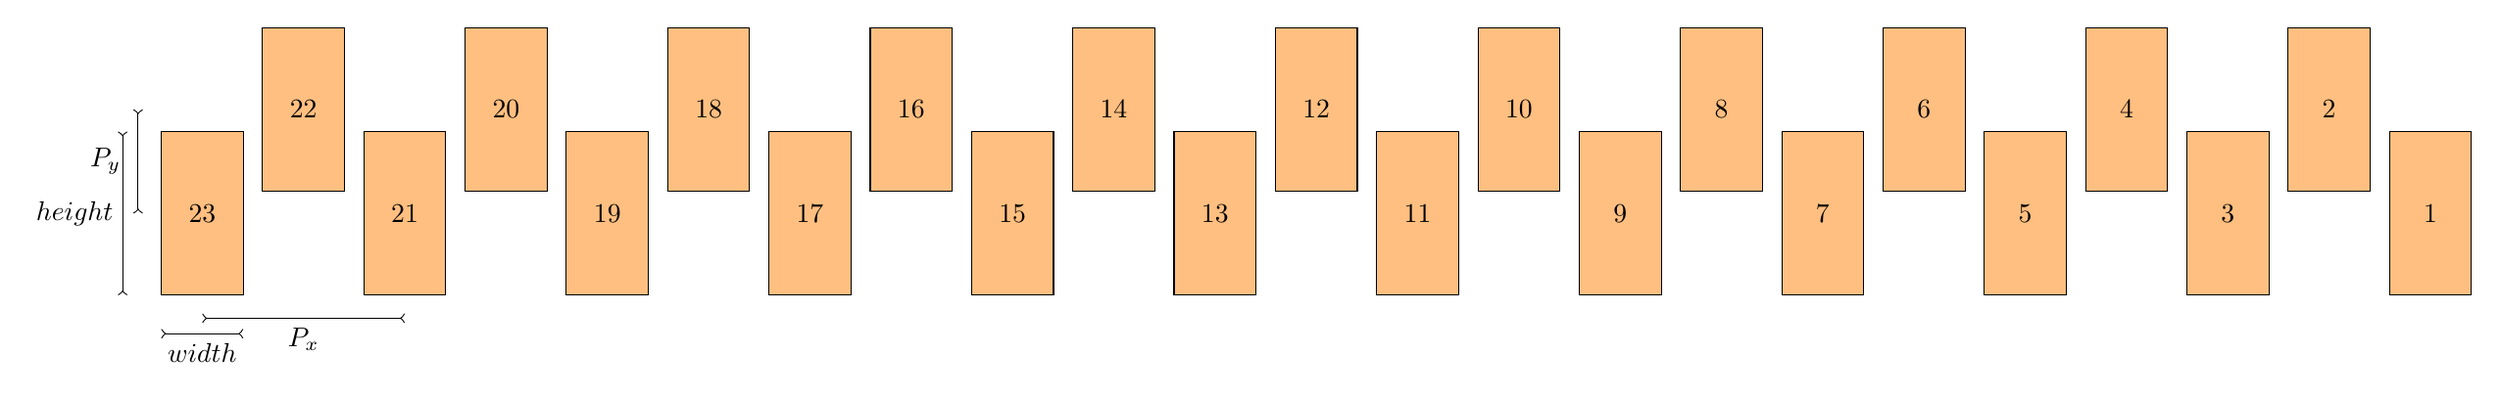
\begin{tikzpicture}

  \def \Px {21/8}
  \def \Py {10.8/8}
  \def \width {8.5/8}
  \def \height {17/8}

  \foreach \i in {0, 1, 2 ,3 ,4 ,5, 6, 7, 8 ,9 ,10, 11}
  {
    \draw[fill=gray!30] (\i * \Px, 0) rectangle (\width + \i * \Px,
    \height);
    \pgfmathtruncatemacro\num{23-2*\i}
    \ifthenelse{\num = 19 \OR \num = 5}{\draw[fill=orange!50] (\i * \Px, 0) rectangle (\width + \i * \Px,
    \height);}{}
    \draw (\width / 2 + \i * \Px, \height / 2) node {\num};
  }

  \foreach \i in {0, 1, 2 ,3 ,4 ,5, 6, 7, 8 ,9 ,10}
  {
   \draw[fill=gray!30] (\Px / 2  + \i * \Px, \Py )
    rectangle (\Px / 2 + \width  + \i * \Px, \Py + \height );
    \pgfmathtruncatemacro\num{22-2*\i}
    \ifthenelse{\num = 14 \OR \num = 10}{\draw[fill=orange!50] (\Px /
      2  + \i * \Px, \Py ) rectangle (\Px / 2 + \width  + \i * \Px, \Py + \height );}{}
    \draw (\width / 2 +\Px / 2 +\i * \Px, \Py + \height / 2) node {\num};
  }

  \draw[>-<] (\width / 2,-.3) -- (\Px + \width / 2,
  -.3);
  \draw (\Px / 2 + \width / 2, -.3) node[below] {$P_x$};
  \draw[>-<] (-.3 , \height / 2) -- (-.3,  \height / 2 + \Py);
  \draw (-.4, \Py /2 + \height / 2) node[left]
  {$P_y$};

  \draw[>-<] (0,-.5 ) -- (\width, -.5);
  \draw (\width / 2, -.5) node[below] {$width$};

  \draw[>-<] (-.5,0) -- (-.5, \height);
  \draw (-.5, \height/2) node[left] {$height$};
\end{tikzpicture}}
\caption{The Zig-Zag array cross section with the numbering
  convention. The four input waveguides  are displayed in orange.}
\label{tikz:ZigZagCrossSection}

\end{figure}
